\begin{center}
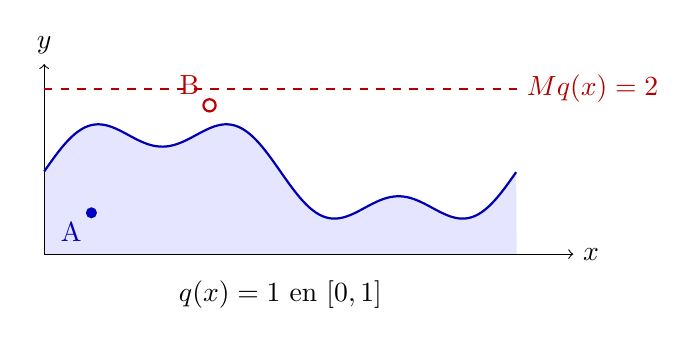
\begin{tikzpicture}[x=6cm,y=1.05cm]
  \fill[blue!10] (0,0) -- plot[domain=0:1,samples=140]
    (\x,{1+0.55*sin(360*\x)+0.25*sin(1080*\x)}) -- (1,0) -- cycle;
  \draw[->] (0,0) -- (1.12,0) node[right] {$x$};
  \draw[->] (0,0) -- (0,2.3) node[above] {$y$};
  \draw[thick,blue!70!black,domain=0:1,samples=140]
    plot (\x,{1+0.55*sin(360*\x)+0.25*sin(1080*\x)});
  \draw[thick,dashed,red!70!black] (0,2) -- (1,2)
    node[right] {$Mq(x)=2$};
  \fill[blue!75!black] (0.1,0.5) circle (2pt) node[below left] {A};
  \draw[red!75!black,thick] (0.35,1.8) circle (2.2pt)
    node[above left] {B};
  \node[below] at (0.5,-0.2) {$q(x)=1$ en $[0,1]$};
\end{tikzpicture}

\small La curva objetivo es $f(x)=1+0.55\sin(2\pi x)+0.25\sin(6\pi x)$.
\end{center}